% 2026-11-04 flow rewrite: plainer words, less repetition; same facts, numbers and \verify items.
% Fig. 1: GaitNet overview. Drawn in Inkscape: edit figures/fig_overview.svg
% and save a PDF copy, with text converted to paths, as
% figures/fig_overview.pdf. Panels: (a) architecture (Sec. III-A, III-B),
% (b) IDM training per controller (III-C), (c) PPO training in Isaac Lab
% (III-D), (d) deployment on OCS2 (III-E).
\begin{figure*}[t]
\centering
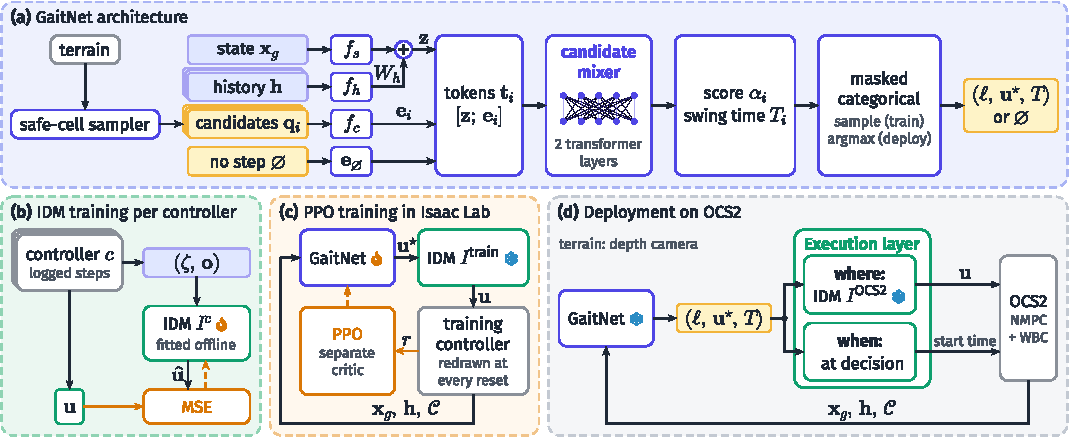
\includegraphics[width=0.87\textwidth]{figures/fig_overview}
\caption{GaitNet overview. (a)~Given the state $\mathbf x_g$ and the
  history $\mathbf h$, a candidate mixer compares the safe candidates
  $\mathbf q_i \in \mathcal C$ and the no-step option $\varnothing$, and
  GaitNet gives each a score and a swing time. (b)~Each controller's IFM
  is fitted offline on logged steps. (c)~PPO training keeps the training
  controller's IFM frozen in the loop. (d)~On OCS2, GaitNet is frozen and
  the execution layer sets the command with the OCS2 IFM. Amber arrows: training signals (solid) and parameter updates
  (dashed). \hot~trained, \frz~frozen.}
\label{fig:overview}
\end{figure*}
